
\chapter{Contesto e Finalità}

Per comprendere nella sua complessità il progetto elaborato in questa
tesi è necessario tenere conto, prima di tutto, del contesto in cui
viene sviluppato e delle finalità implicite ed esplicite che si vogliono
raggiungere. Si tratta di descrivere lo sviluppo di un applicativo
mobile fortemente legato ai sistemi di marketing e alle nuove strategie
di business di aziende leader all'interno dei propri mercati, in molti
casi saturi o fortemente instabili, scossi dalle innovazioni tecnologiche
di questi decenni.

Oltre alle ingerenze esterne sul progetto, come il cambiamento repentino
delle tecnologie o la presenza di eventuali competitor, deve essere
valutata la posizione del singolo componente all'interno dello sviluppo
dell'interno progetto, la quale va tenuta in forte considerazione
specialmente durante la prima fase di sviluppo in cui si determinano
le prime linee guida da seguire durante tutto il lavoro.

Questo elaborato rientra nel concetto di \textit{Application Economy},
che descrive perfettamente il trend degli ultimi anni. Il cambiamento
dei metodi con cui le masse ottengono informazioni e si lasciano influenzare
hanno portato a un sostanziale sconvolgimento del sistema di marketing
e delle strategie commerciali anche di aziende multinazionali, spostando
l'interesse sulla ricerca nel campo delle applicazioni mobile. Proprio
in questo contesto è necessario inquadrare le motivazioni che hanno
portato Carpigiani, azienda leader nel settore della produzione di
macchine per il gelato, a dare vita all'ecosistema MyGelato, di cui
questa tesi sviluppa solo una componente, valutando sia le finalità
in ambito di marketing sia in ambito commerciale e produttivo.

\section{Application Economy}

\begin{figure}[h]
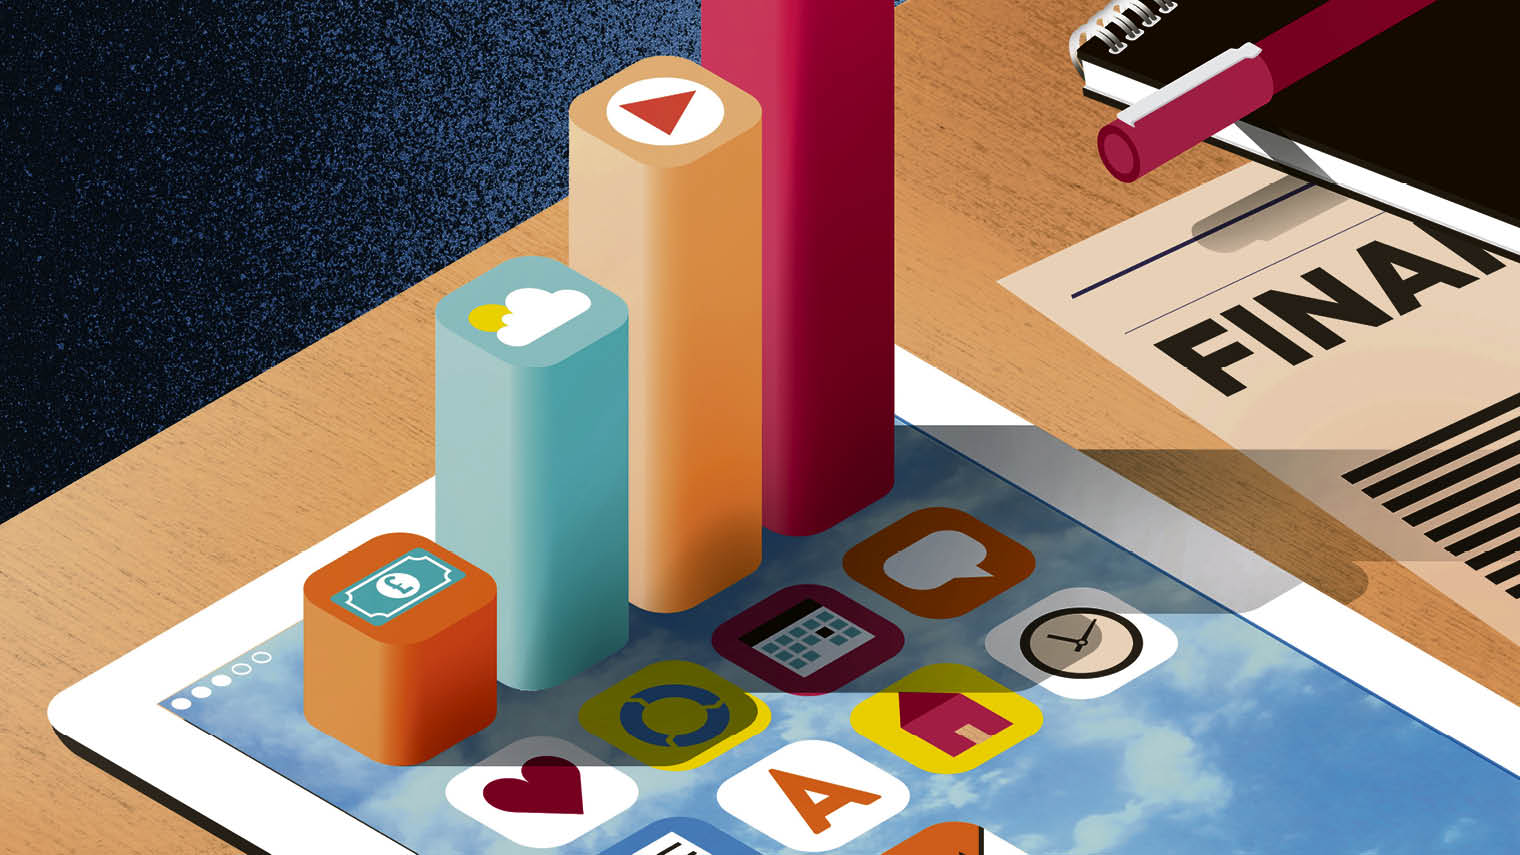
\includegraphics[width=1\linewidth]{/home/tommaso/Documents/Tesi/thesis/images/The-App-Economy}
\caption{Application Economy}
\label{fig:appEconomy1} 
\end{figure}

Non vi è forse modo di descrivere la società attuale e questo periodo
storico senza valutare l'importanza dello sviluppo tecnologico che
ci ha portato in quella che viene definita l'\textit{Era dell'Informazione}.
La rivoluzione tecnologica che sta avvenendo in questi anni, specialmente
a partire dagli anni Novanta, ha portato la connessione globale a
Internet ad assumere un ruolo essenziale in ogni aspetto della società
moderna e della nostra vita.

È cambiato drasticamente il modo con cui le persone accedono alle
informazioni, che siano queste di tipo personale o di tipo commerciale.
Allo stesso modo si sono dovute adeguare le strategie di tutte quelle
aziende che hanno visto cambiare in maniera drastica il proprio mercato,
invaso molte volte da tecnologie sempre più diversificate e innovative.\bigskip{}

Secondo il giornalista Paul Mason, è stata la dottrina economica degli
ultimi decenni della nostra epoca che da una parte ha avuto il merito
di promuovere la più grande ondata di sviluppo economico che il mondo
abbia mai visto, ma dall’altra ha portato a mercati incontrollati
e a vorticosi cambiamenti sociali innescati dalla tecnologia. Si sono
diffusi, infatti, concetti come i progetti open-source, la sharing
economy e le licenze creative commons che hanno messo in crisi le
fondamenta del capitalismo odierno. Questo fenomeno unito alla saturazione
di molti mercati ha portando tante aziende a dover rivedere la propria
business strategy obbligandole a dirigere i propri investimenti sulla
diversificazione e sulle nuove strategie di vendita. \cite{POSTCAPITALISMO}

\bigskip{}

C'è stato un cambio di paradigma per tutti i meccanismi di commercializzazione
di un prodotto: sono diventati di fondamentale importanza i concetti
di \emph{e-commerce} e \emph{marketing digitale}, fortemente spinti
dalle tecnologie e dalla nuova possibilità di accedere a una risorsa
comune (Internet) da parte della maggior parte della persone anche
di cultura, età e ambienti sociali diversi. L'utente medio, per esempio,
viene ormai maggiormente raggiunto e conivolto tramite email pubblicitarie
o advertising online rispetto a meccanismi tradizionali ormai meno
incisivi di marketing non digitale.

\bigskip{}

Legato alla diffusione sempre crescente di smartphone, che sono di
fatto diventati l'accesso principale degl utenti a Internet, nasce
quindi l'\textit{Application Economy}: lo sviluppo e l'utilizzo di
applicazioni mobile per raggiungere e dialogare tramite un collegamento
bidirezionale con i consumatori. Tramite un applicativo mobile è quindi
possibile svolgere una serie di azioni online in mobilità e con semplicità;
potendo confidare, nella maggior parte dei casi, in un'alta sicurezza
della propria connessione e nello scambio dei dati.

Se questa strategia può essere applicata, per esempio, in ambito marketing
per pubblicizzare un proprio prodotto e fidelizzare il consumatore
alla propria azienda, è forse più incisivo osservare come l'e-commerce
abbia ormai soppiantato la commercializzazione tradizionale in molti
ambiti, specialmente tramite applicativi mobile (una statistica del
BI Intelligence riporta che entro il 2020 il commercio mobile supererà
il 45\% degli acquisti online complessivi). L'abbattimento dei costi
di un rivenditore non fisico e la nascita di servizi di pagamento
online come PayPal hanno portato questa rivoluzione in ogni ambito
commerciale permettendo, inoltre, all'utente di pagare direttamente
tramite sistemi bancari online in sicurezza e con semplicità.\bigskip{}

Tutti questi concetti sono ormai più che affermati in ambiti come
la vendita di prodotti di abbigliamento o tecnologici, ma l'azienda
Carpigiani ha scelto di portare questi nuovi meccanismi anche all'interno
della vendita di Gelati, in modo innovativo e fortemente avanti nei
tempi grazie al progetto \emph{MyGelato}.

\section{Ecosistema MyGelato}

L'ecosistema MyGelato si pone all'interno del contesto descritto nel
capitolo precedente, a unire le strategie di marketing dell'azienda
produttrice Carpigiani e delle singole gelaterie convenzionate: una
piattaforma web e mobile che si rivolge ai gelatieri e ai consumatori
di gelato. Gli obiettivi commerciali sono diversi, primi tra i quali
quello di incentivare la compravendita di gelati tramite un sistema
di coupon digitali e quello di promuovere il consumo di gelato tramite
offerte, fornendo anche ai gelatieri un sistema semplice ed efficace
per pubblicizzare il proprio negozio.\bigskip{}

Attraverso l'applicativo, l'utente può informarsi sulle gelaterie
presenti in zona verificando anche quali facciano parte del circuito
MyGelato: insieme delle gelaterie convenzionate alla vendita e alla
validazione dei coupon online. È possibile ottenere alcune informazioni
utili, come indirizzo e numero di telefono, salvarle nei preferiti
e verificare se vi sono promozioni attive. Sono strategie ovviamente
di carattere pubblicitario e permettono anche a gelaterie minori,
facenti però parte del circuito, di essere pubblicizzate agli utenti
che utilizzano la piattaforma.

Questo sistema permette all'azienda Carpigiani di avere un controllo
maggiore su un sistema centralizzato di advertasing per le gelaterie
di cui è principale fornitore, ottenendo quindi la possibilità di
intervenire su realtà locali standardizzandone alcuni meccanismi.\bigskip{}

Seconda feature fondamentale dell'applicazione, che riguarda in questo
caso solo gli utenti iscritti al sistema, è la possibilità di comprare
online dei coupon digitali che permettono l'acquisto di un gelato
presso una determinata gelateria. Questi coupon sono visualizzabili
in ogni momento e possono essere regalati anche ad altri utenti tramite
un semplice metodo di condivisione che permette al destinatario di
usufruire dell'oggetto comprato. Ogni gelateria che supporta questo
sistema sarà provvista della stessa applicazione con un account specifico
per il gelatiere che permetterà di validare i coupon utilizzati e
ricevere il proprio compenso tramite il sistema di pagamento online.

Questo sistema di e-commerce sposta la vendita di un prodotto molto
semplice come i gelati, online. È infatti possibile comprarli tramite
carta di credito e l'azienda Carpigiani, nel frattempo, si inserisce
in un meccanismo legato a delle realtà locali sul quale altrimenti
non riuscirebbe ad avere informazioni. Questo sistema, per quanto
diffuso in altri mercati come il reselling online di oggettistica
è fortemente innovativo in questo campo e rende l'ecosistema MyGelato
uno dei primi nel suo settore.

\begin{figure}[h!]
\centering{}
\includegraphics[scale=0.4]{/home/tommaso/Documents/Tesi/thesis/images/mygelato}
\caption{Logo MyGelato}
\end{figure}

\newpage{}
